% LaTex文档的基本结构、编译和调试、命令符号的输入(如%,{..}等等)
\documentclass{book} %book,report,letter
% 在\documentclass{artical}和begin{document}之间的部分被称为导盲区
\usepackage{amsmath} %宏包,美国数学协会
\usepackage{mathrsfs}
\usepackage{arydshln}
\usepackage{graphicx}

\begin{document}
% 正文部分
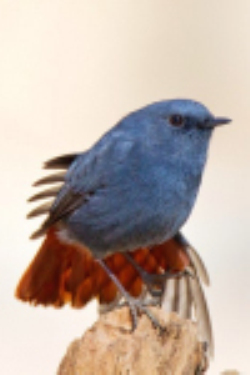
\includegraphics{pic1.jpg}
\begin{figure}
\centering
	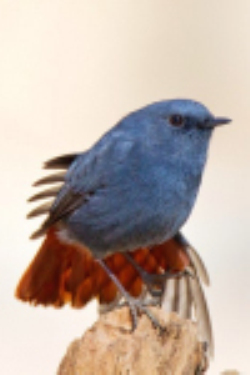
\includegraphics[scale=1,angle=30]{pic1.jpg}
	\caption{this is a tu}
\end{figure}
\end{document}

